\chapter{Negative pulse events}
\label{cha:np}
During the operation of Siegfried II inside the Gerdalinchen II (GII)
test stand (see Chapter~\ref{cha:GII}), a peculiar class of events was
observed in significant numbers. The pre-amplifiers and the DAQ system
were configured such, that all channels had positive polarity,
\textit{i.e.}, all signal pulses had to be positive. About 5\% of the
events nevertheless had in at least one segment a negative baseline
shift that could be interpreted as a ``negative pulse''.

\section{An example}
\label{sec:np:evt}
Figure~\ref{fig:np:npul} shows a typical negative pulse event. In this
single-segment event all the energy was deposited in segment 1. The
neighboring segments all show mirror pulses as expected from the
weighting potentials. Almost all other segments, however, show some
negative baseline shifts. In the following the phenomenon is
investigated and an explanation proposed.

\begin{sidewaysfigure}[htbp]
\centering
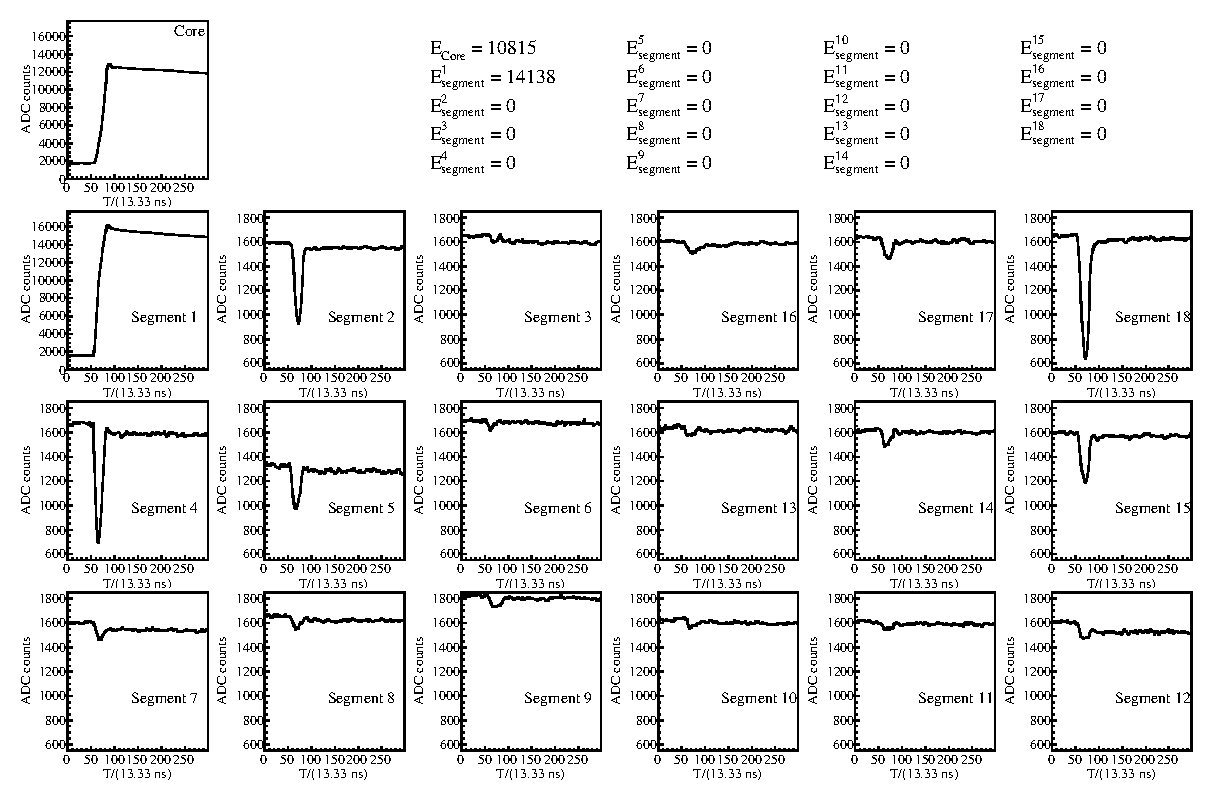
\includegraphics{npul}
\caption{An single-segment event with energy deposited in segment 1
showing negative baseline shifts in almost all other segments. Mirror
pulses are observed as expected.}
\label{fig:np:npul}
\end{sidewaysfigure}


\section{Selection of negative pulse events}
\label{sec:np:sel}
If the energies of negative pulses are correctly calculated, the sum
of the the energies seen in all segments, $\sum E_{\text{segment}}$,
is equal to the core energy, $E_{\text{core}}$, within the
resolution. The DAQ system, However, sets the energy of a negative
pulse to zero instead of a negative value, this causes $\sum
E^{\text{DAQ}}_{\text{segment}}$ to be larger than $E_{\text{core}}$.

Figure~\ref{fig:np:sEnegPulse} shows $\sum
E^{\text{DAQ}}_{\text{segment}}$ versus $E_{\text{core}}$ of a data
sample collected with a $^{228}$Th source mounted inside GII on top of
Siegfried II. The two solid lines in the plot indicate the $\pm 10
\sigma$ range around the core energy. Points above the upper solid
line correspond to the negative pulse events, which were selected by
requiring $\sum E^{\text{DAQ}}_{\text{segment}} - E_{\text{core}} >
10\sigma$.

\begin{figure}[tphb]
\centering
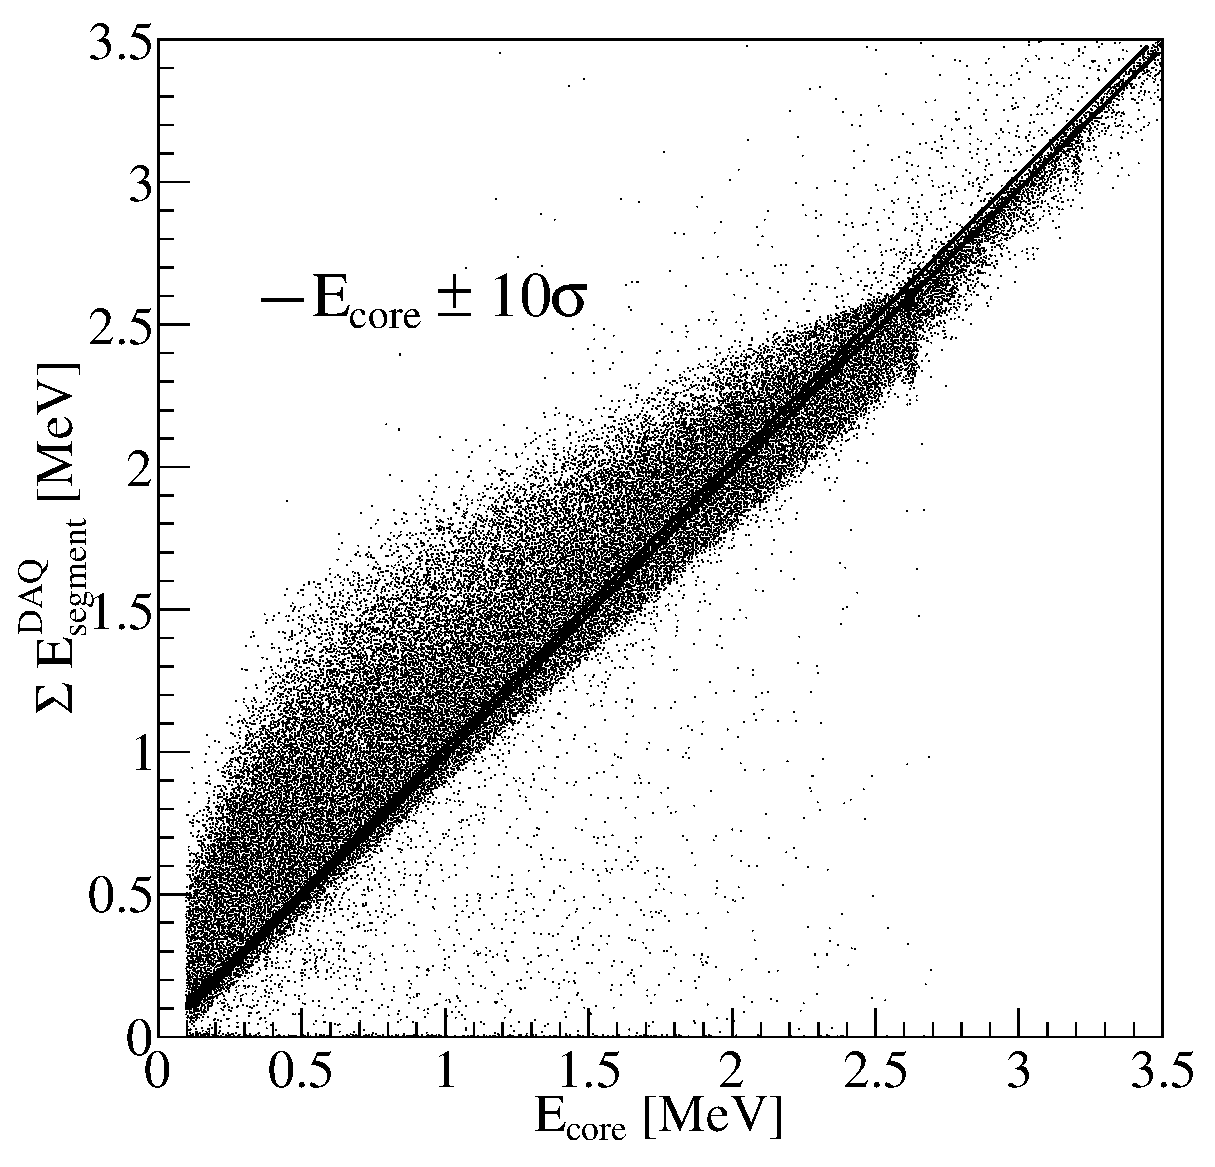
\includegraphics[width=0.5\textwidth]{sEnegPuls}
\caption{Sum of segment energies as determined by the DAQ versus the
core energy. The two solid lines indicate the 10$\sigma$ range around
the core energy.}
\label{fig:np:sEnegPulse}
\end{figure}

There is also a small fraction of events with$\sum
E^{\text{DAQ}}_{\text{segment}} < E_{\text{core}}$. This is due to
threshold-effects, noise or pile-up, \textit{i.e.} two pulses are
spaced in time such that the DAQ cannot provide a correct estimate of
the core and segment energies. As there are quite a number of events
with an energy beyond 2.6~MeV, the pile-up effects are probably
significant.

\section{Location of negative pulse events}
\label{sec:np:locneg}
To localize the effect, the individual segment energies were plotted
versus the core energy for the selected
events. Figure~\ref{fig:np:EnegPulse} shows that predominantly the top
and bottom segments feature the case $E^{\text{DAQ}}_{\text{segments}} >
E_{\text{core}}$. Very few negative pulse events were found in the
segments in the middle of the detector.
 
\begin{sidewaysfigure}[tphb]
\centering
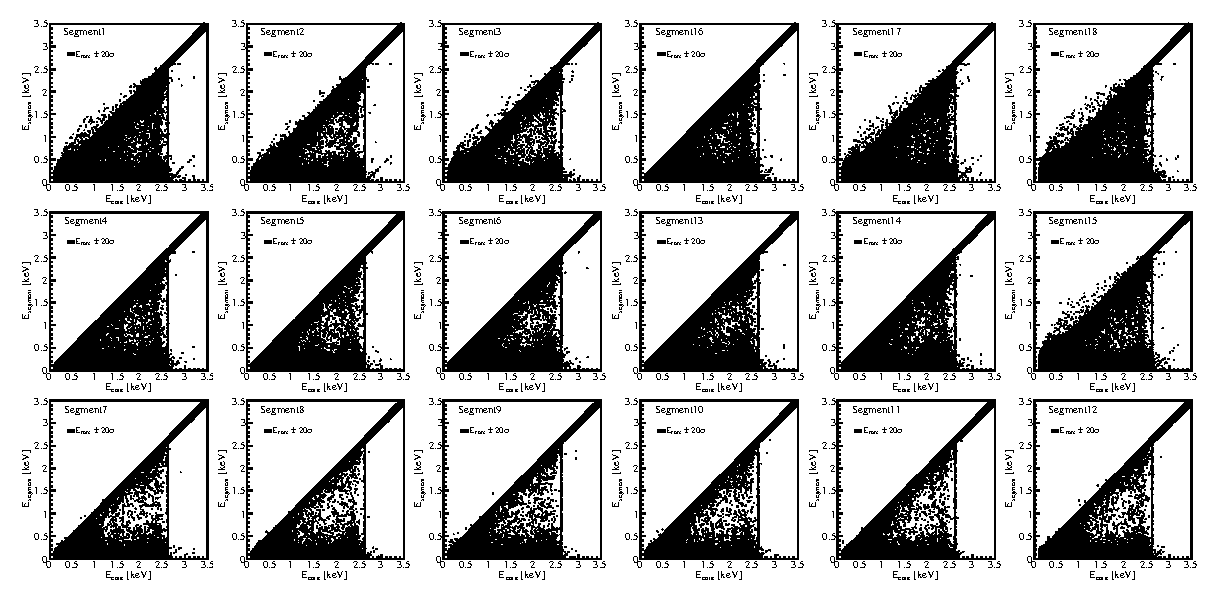
\includegraphics{EnegPuls}
\caption{Energies of individual segments versus the core energy. All
energies were calculated by the DAQ system. The two solid lines in
each plot indicate the $\pm 10 \sigma$ range around the core energy.}
\label{fig:np:EnegPulse}
\end{sidewaysfigure}

Table~\ref{tab:np:nenum} lists for each segment the total number of
affected single segment events and the percentage it represents. The
position of the source (above the detector) is clearly reflected in
the differences of numbers of events between top and bottom segments.
The percentage of affected events seems relatively constant for all
segments of a layer. The bottom segments have a lower percentage of
affected events than the top segments.

\begin{table}[tbhp]
\centering
\caption{Number of single segment negative pulse events. Given are 
absolute numbers and the percentage of single segment events
they represent.}
\label{tab:np:nenum}
\scriptsize
\begin{tabular}{l|rrr|rrr|r} \hline
Top  & 1 & 2 & 3 & 16 & 17 & 18 & total \\\hline
Number ($10^{3}$) &$88.5\pm0.3$&$61.2\pm0.2$&$90.7\pm0.3$&$133.6\pm0.4$&$89.0\pm0.3$&$102.7\pm0.3$&$565.7\pm0.8$\\ 
Percentage (\%) &$5.34\pm0.02$&$5.28\pm0.02$&$7.31\pm0.03$&$9.24\pm0.03$&$5.47\pm0.02$&$5.73\pm0.02$&$6.34\pm0.01$\\
\hline Middle& 4 & 5 & 6 & 13 & 14 & 15 & total \\\hline
Number ($10^{3}$) &$1.25\pm0.04$&$1.15\pm0.03$&$0.97\pm0.03$&$1.49\pm0.04$&$2.15\pm0.05$&$1.73\pm0.04$&$8.74\pm0.09$\\ 
Percentage (\%) &$0.22\pm0.01$&$0.28\pm0.01$&$0.21\pm0.01$&$0.26\pm0.01$&$0.34\pm0.01$&$0.24\pm0.01$&$0.26\pm0.01$\\
\hline Bottom& 7 & 8 & 9 & 10 & 11 & 12 & total \\\hline
Number ($10^{3}$) &$18.1\pm0.1$&$11.5\pm0.1$&$15.8\pm0.1$&$14.4\pm0.1$&$13.2\pm0.1$&$17.6\pm0.1$&$90.6\pm0.3$\\ 
Percentage (\%) &$3.46\pm0.03$&$3.05\pm0.03$&$3.69\pm0.03$&$2.94\pm0.02$&$2.38\pm0.02$&$2.79\pm0.02$&$3.02\pm0.01$\\ \hline 
\end{tabular}
\end{table}

To investigate whether the events are concentrated at a particular
radius, the risetimes of the events were studied.
Figure~\ref{fig:np:nert} shows the distribution for normal and
negative pulse events. The distribution for negative pulse events is
significantly shifted toward higher risetimes. However, as the
risetimes above $\approx 400$~ns are in principle unphysical, this is
probably not an indication that the events are located at very large
or very small radii, but rather that they are located in regions where
the electric field is not at full strength. Such regions can exist
close to the top and bottom surfaces of the detector.

\begin{figure}[tphb]
\centering
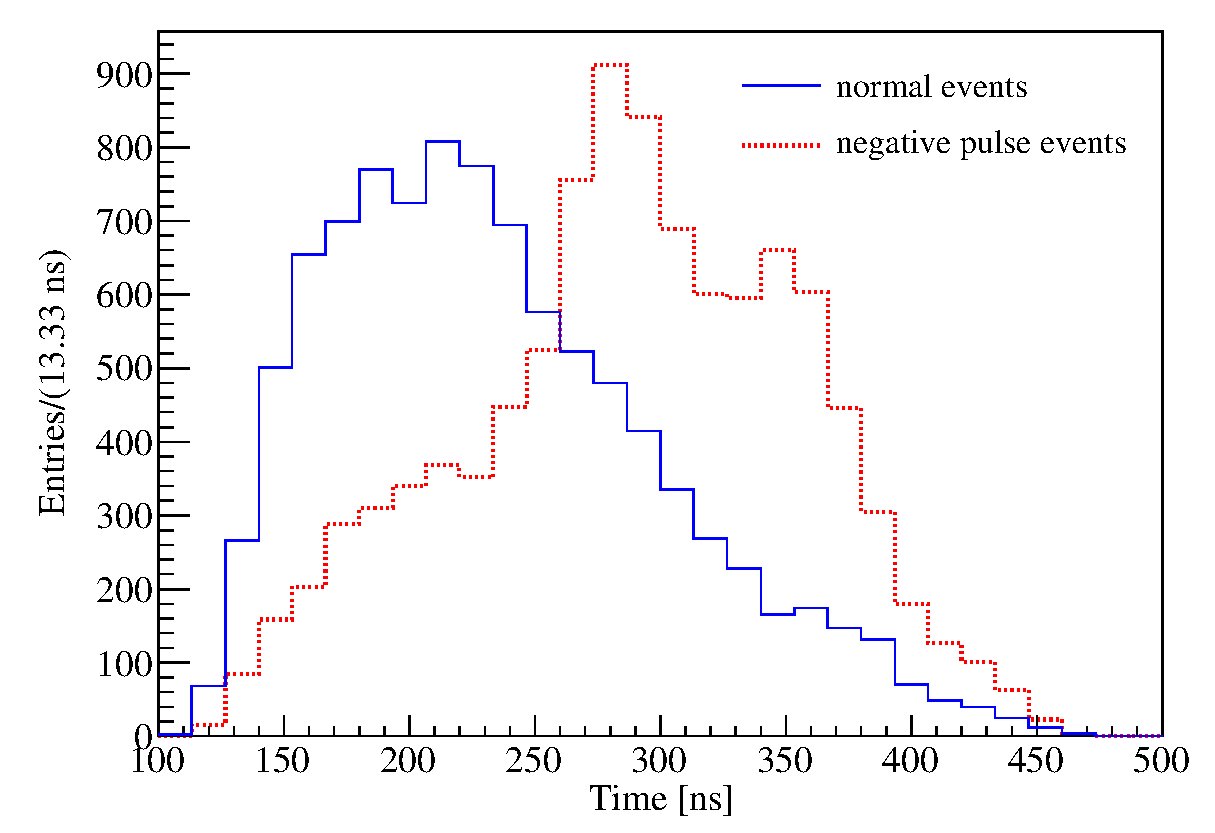
\includegraphics[width=0.6\textwidth]{RTall}
\caption{Core risetime distribution of normal and negative pulse events.}
\label{fig:np:nert}
\end{figure}

\section{Explanation}
\label{sec:np:exp}
The end surfaces of true-coaxial detectors have a priori undefined
potential. The formation of surface channels \cite{Sur05} and the
deformation of the electric field are expected. The charge carriers
slow down and might even get trapped near the end surfaces. The
trapping of electrons leads to a reduction of the signal both in the
core and in the segment containing the hit. However, as the core is
mainly sensitive to the drift of the electrons, it is affected
stronger than the segment which is mainly sensitive to the drift of
holes. As a result a given photon peak in the core energy spectrum
would show a large shoulder at lower energies. However, such a
shoulder can also occur, if the pulses are just too long, because the
DAQ energy filter does not handle extremely long risetimes correctly
and calculates an energy slightly smaller than the full energy. Such a
shoulder was already observed in data collected with Siegfried~I (see
Fig.~\ref{fig:np:shou}): the low energy side of the 1332~keV peak from
$^{60}$Co is significantly higher than in the simulation assuming no
field distortion.

\begin{SCfigure}[][htbp]
\centering
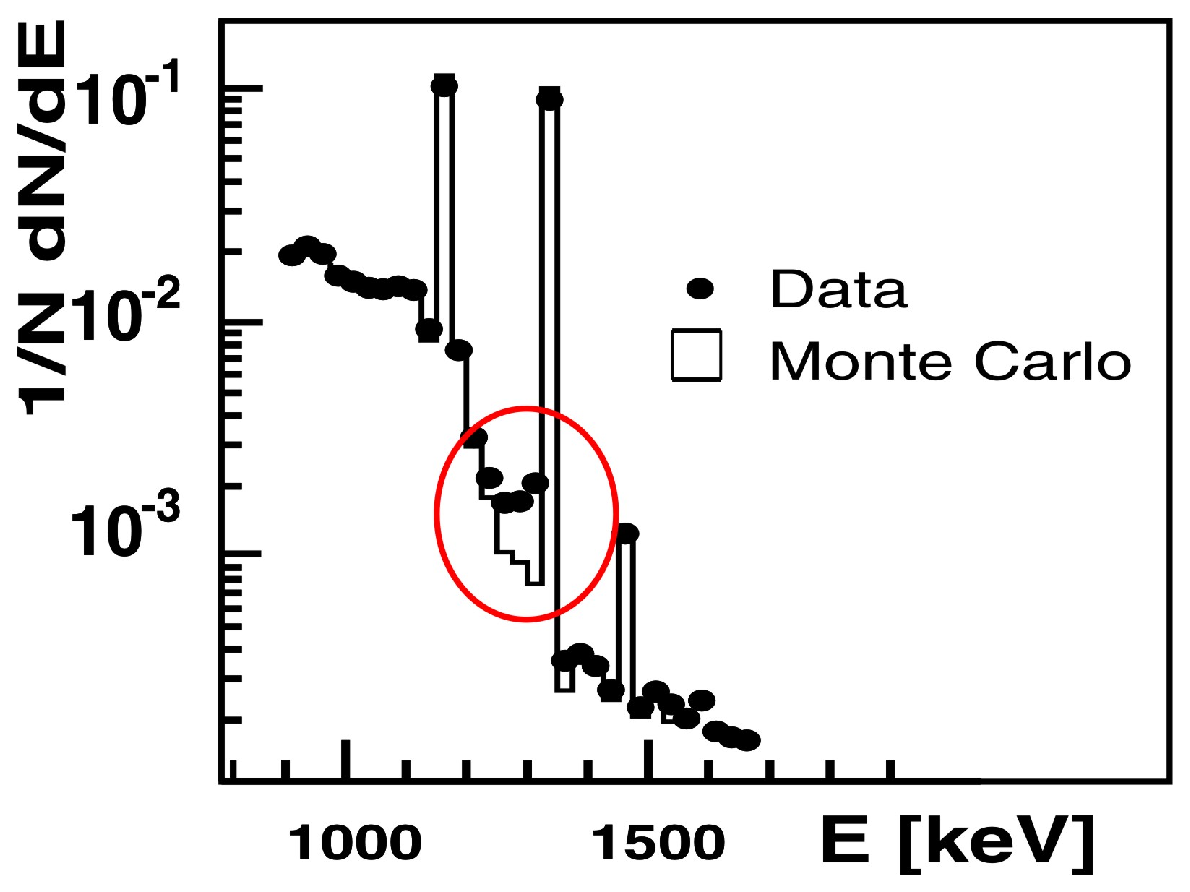
\includegraphics[width=0.4\textwidth]{dmcnew}
\caption{A slice of core energy spectrum around 1332~keV peak taken
with Siegfried~I. The low energy side of the 1332~keV peak in data is
significantly higher than in the simulation.}
\label{fig:np:shou}
\end{SCfigure}

If the pulse gets longer and longer, \textit{i.e.} the field becomes
very small, the electrons are effectively trapped and the mirror pulse
in a neighboring segment cannot be completed resulting in an effective
negative baseline shift, \textit{i.e.} negative pulse.

\section{Surface investigation}
\label{sec:np:inv}
If indeed negative pulse events are located close to the end surfaces
of the detector, the low energy part of the spectrum should be
especially affected. Figure~\ref{fig:np:fracall} shows the fractions
of single segment negative pulse events for all 18 segments versus the
core energy as determined by the DAQ system. In all top and bottom
segments a rising fraction is seen below 100~keV. Also seen are
relatively large fractions just below the 2614~keV photon peak from
$^{208}$Tl. This would lead to a shoulder in the spectrum as described
in the previous section.

\begin{sidewaysfigure}
\centering
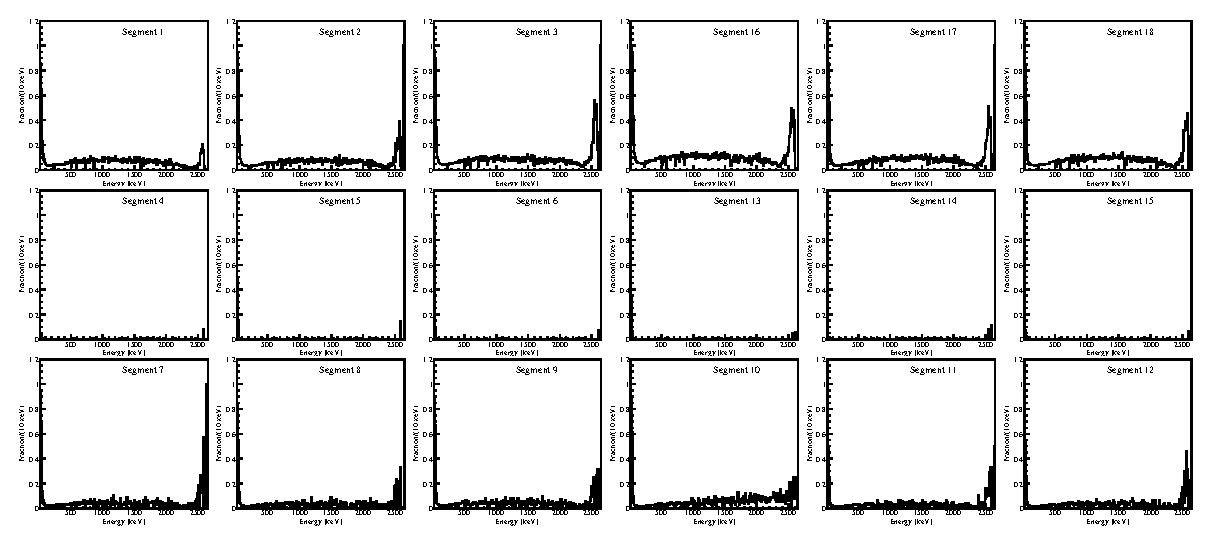
\includegraphics{NegFractionAll}
\caption{Fraction of single segment negative pulse events as a
function of core energy in all segments.}
\label{fig:np:fracall}
\end{sidewaysfigure}

\begin{figure}[tphb]
\centering
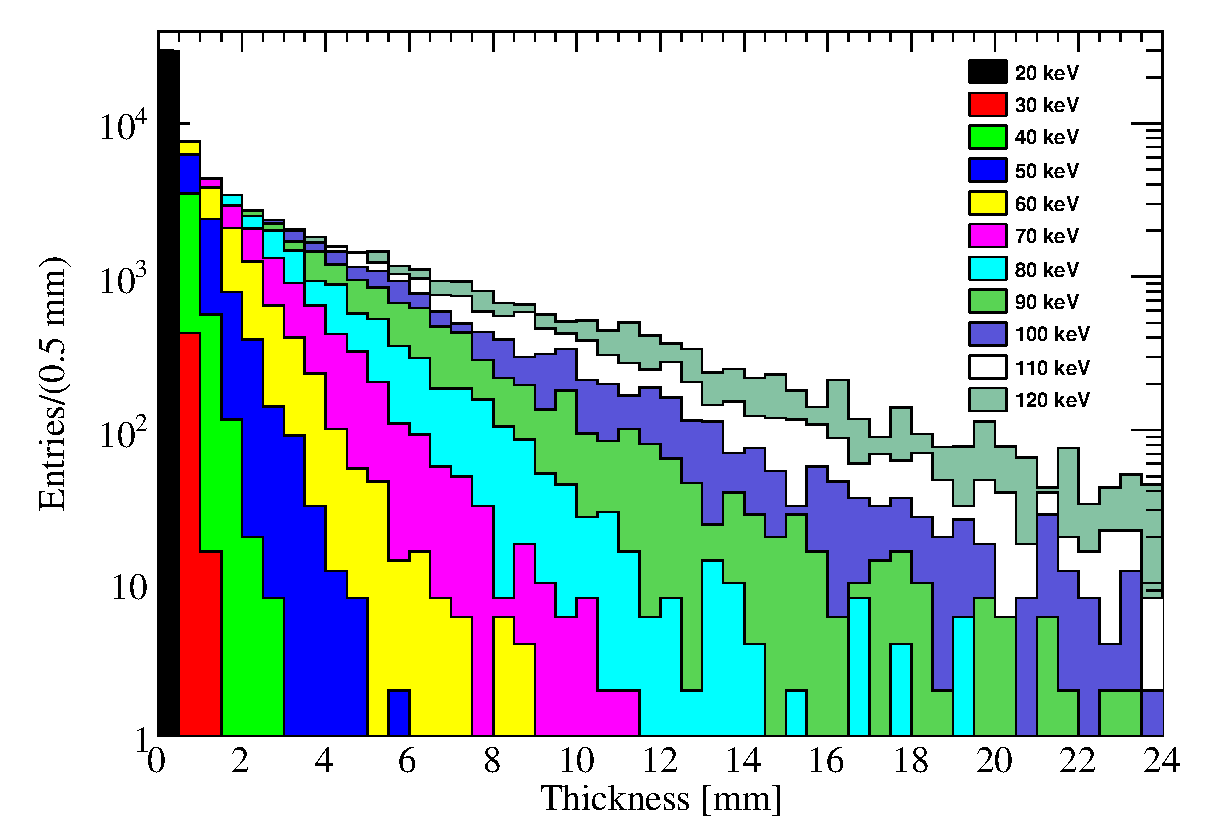
\includegraphics[width=0.6\textwidth]{gDepth}
\caption{Depth distributions of hits created by low energy photons
entering the detector form the top.}
\label{fig:np:gdep}
\end{figure}

The top surface of the detector is illuminated best with low energy
photons. The penetration of low energy photons into germanium is shown
in Fig.~\ref{fig:np:gdep}. Photons with an energy of 20~keV are all
absorbed within the first 0.5~mm of the detector. The penetration
power of photons increase rapidly with energy. Only about 15\% of the
100~keV photons are absorbed there. Thus the fraction of events with
negative pulses should rapidly decrease with energy. This is shown in
Fig.~\ref{fig:np:fraclow} for a top and a middle segment. While the
middle segment shows only a very small and statistically uncertain
effect the top segment gives a clear indication of a decreasing
fraction of events affected. The distribution flattens out at about
100~keV. The fraction of events at this energy is $\approx 5\%$. This
corresponds to a penetration of about 200~$\mu$m.

\begin{figure}[tphb]
\centering
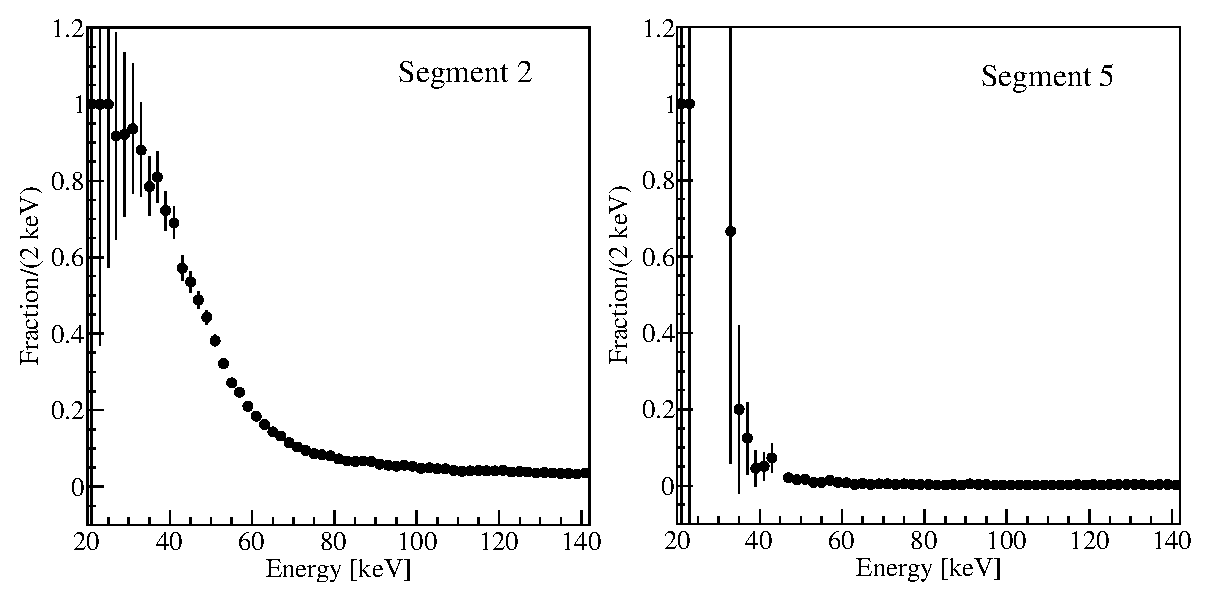
\includegraphics[width=0.95\textwidth]{NegFraction20140}
\caption{Fraction of single segment negative pulse events in the low
energy region for segment~2 in the top layer and segment 5 in the
middle layer.}
\label{fig:np:fraclow}
\end{figure}

Figure~\ref{fig:np:frac2614} shows the situation near the $^{208}$Tl
line at 2614~keV. The negative pulse events show up as a large fraction
below the line energy. This enhancement is seen down to about 2400~keV,
\textit{i.e.} up to 200~keV energy can get lost. The fraction of
events shifted is about 1\%. As the distribution of hits created by
2614~keV photons is basically homogeneous this directly translates into
a volume corresponding to a surface layer of $\approx 200 \mu$m.

\begin{figure}[tphb]
\centering
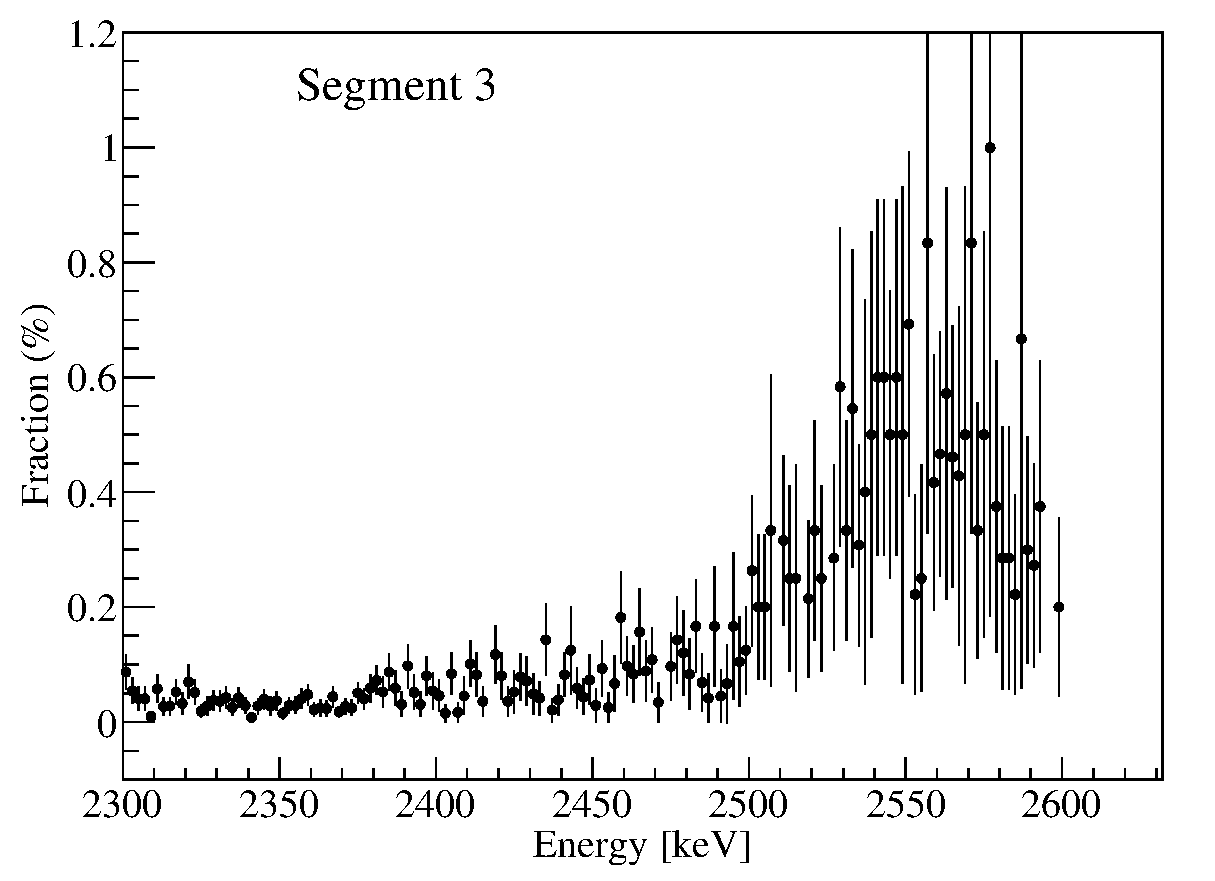
\includegraphics[width=0.6\textwidth]{NegFraction2614}
\caption{Fraction of single segment negative pulse events on the low
energy side of 2614~keV peak.}
\label{fig:np:frac2614}
\end{figure}

The different approximation indicate that Siegfried~II has a surface
layer with a thickness of about 200~$\mu$m where the electric field is
distorted. This is smaller than what was claimed by a previous
publication \cite{Ebe08}. However, this publication refers to a very
different detector. The effect for Siegfried~I was much smaller,
indication that it had a thinner layer of field distortion. This is
probably due to the fact that Siegfried~I has fully metalized segment
surfaces while Siegfried~II only has relatively small metal contacts.

The events can be clearly identified through the pulse shapes. Thus,
this can actually be used to define a fiducial volume of the detector
and to reject surface events.

\section{Summary}
\label{sec:np:sum}
A special class of events with negative baseline shifts was traced to
interactions close to the end surfaces of the detector. The rate of
such events for Siegfried~II indicates a layer with a distorted
electric field of about 200~$\mu$m depth. As the events can be clearly
identified they can be used to characterize the fiducial volume of a
given detector and they can be used to identify surface events. This
might be of help in reducing the background from $\alpha$-sources.

%%% Local Variables:
%%% mode:latex
%%% TeX-master: "thesis"
%%% End:
